\question{\bfseries Descending Drills}

\subsection*{\sectionfont\upshape Background}

ผืนดินแห่งหนึ่งมีสมบัติซ่อนอยู่ใต้ดินมากมาย เนื่องด้วยเทคโนโลยี Remote Sensing ในปัจจุบัน
ทำให้เราสามารถสำรวจมูลค่าของสมบัติที่อยู่ใต้ดินในบริเวณต่าง ๆ ได้ 
โดยที่เราไม่ต้องขุดสมบัติออกจากดินเพื่อมาตีราคาแต่อย่างใด

เราจะมองชั้นดินที่เต็มไปด้วยสมบัติดังกล่าวเป็นพื้นที่หน้าตัดรูปสี่เหลี่ยมผืนผ้า 
ซึ่งเราจะแบ่งสี่เหลี่ยมผืนผ้าดังกล่าวเป็นชั้นดินลึก $R$ ชั้น ชั้นละ $C$ ช่อง 
ดินแต่ละช่องจะมีมูลค่าของสมบัติกำกับไว้ด้วยซึ่งเป็นจำนวนเต็มที่อาจเป็นบวก ลบ หรือศูนย์ก็ได้

\bigskip\noindent
\textbf{\uline{ตัวอย่าง}} รูปต่อไปนี้คือตัวอย่างข้อมูลของสมบัติในชั้นดินที่มี $R = 6$ และ $C = 6$
\begin{center}
    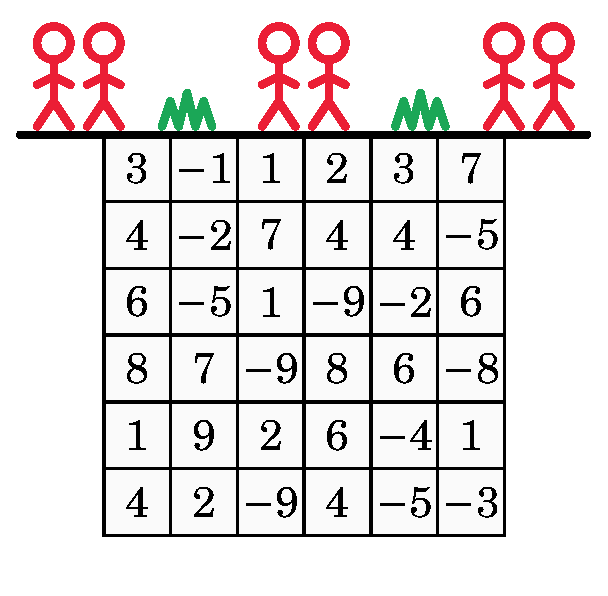
\includegraphics[scale=0.6]{figures/coding_descendingdrills_01.eps}
\end{center}

\subsection*{\sectionfont\upshape Drilling Constraints}
เราต้องการจะเจาะผืนดินเพื่อล่าสมบัติที่อยู่ในดินให้ได้ผลรวมมากที่สุด แต่เนื่องด้วยขีดจำกัดของนวัตกรรมการขุดเจาะที่ยังมีราคาแพง ทำให้เรามีโอกาสเดียวเท่านั้นในการขุดเจาะผืนดินดังกล่าว ลักษณะเส้นทางของการขุดดินจะมีเงื่อนไขดังนี้
\begin{itemize}
\item เราสามารถเริ่มต้นขุดเจาะจากผิวดิน เหนือช่องคอลัมน์ใดก็ได้
\item ตลอดการขุดเจาะในครั้งนี้ เราสามารถขุดเจาะดินในแนวดิ่ง 
    เผื่อลงไปยังชั้นดินชั้นต่อไปก็ได้ หรือจะขุดเจาะในแนวราบไปทางซ้ายหรือขวาในชั้นดินระดับเดียวกันก็ได้ 
    แต่ไม่สามารถเจาะสวนทางแรงโน้มถ่วงในทิศทางชี้สู่ผิวดินได้
\item สำหรับการขุดเจาะแนวราบนั้น เมื่อเราขุดเจาะลงสู่ชั้นดินหนึ่ง ๆ 
    เครื่องขุดเจาะอาจจะเลือกขุดเจาะไปทางซ้ายหรือทางขวา ทิศทางใดทิศทางหนึ่งเท่านั้น 
    (หรือจะไม่ขยับในแนวราบก็ได้) และการขุดแนวราบดังกล่าว จะขยับจากจุดเริ่มต้นได้ไม่เกิน $K$ ช่อง
\item เครื่องขุดเจาะไม่สามารถเดินถอยหลังไปยังช่องดินที่เคยขุดเจาะไปแล้วได้ ไม่ว่าจะเป็นแนวดิ่งหรือแนวราบก็ตาม
\item การขุดเจาะจะสิ้นสุดที่ช่องใดก็ได้\;
    และมูลค่ารวมของสมบัติที่เก็บสะสมได้ คือผลรวมของมูลค่าของสมบัติทุกช่องที่เครื่องขุดเจาะนี้แทรกผ่าน

\item ไม่จำเป็นว่าจะต้องขุดเจาะถึงชั้นผิวดินแถวล่างสุดเสมอไป
\item สมบัติที่มีมูลค่าติดลบที่ค้นพบระหว่างทางจะต้องถูกนำมารวมในผลรวมด้วยเสมอ
\item หากไม่มีรูปแบบการขุดเจาะที่ทำให้ผลรวมสมบัติเป็นบวกเลย สามารถตอบ \verb|0| ได้
\end{itemize}

\bigskip\noindent
\textbf{\uline{ตัวอย่าง}} รูปต่อไปนี้มีเส้นสีส้มแสดงเส้นทางการขุดเจาะชั้นดิน เพื่อล่าสมบัติที่อยู่ในดิน\;
โดยมีเงื่อนไขว่า $K=2$ สังเกตว่าไม่มีการขยับในแนวราบเกิน 2 ช่องเลยในทุกระดับชั้นดิน

ผลรวมมูลค่าสมบัติที่ขุดเจาะตามเส้นทางตัวอย่างนี้คือ 63 หน่วย ซึ่งเป็นเส้นทางที่ดีที่สุดสำหรับรูปตัวอย่างนี้
\begin{center}
    \vspace*{-1.5\baselineskip}
    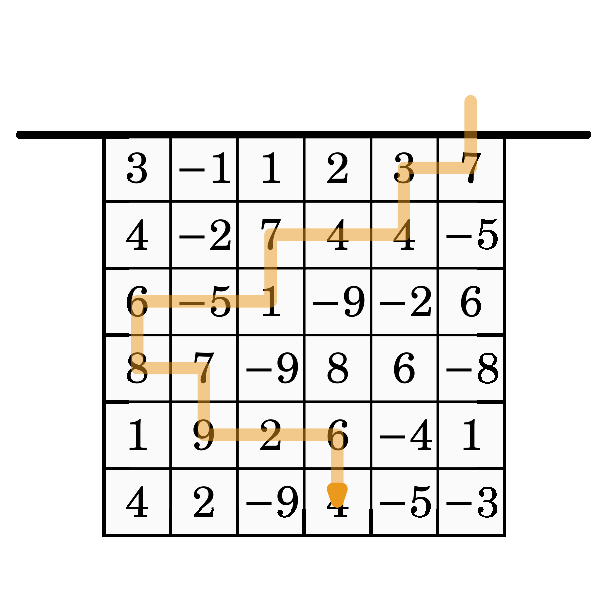
\includegraphics[scale=0.6]{figures/coding_descendingdrills_02.eps}
\end{center}

\subsection*{\sectionfont\upshape Problem Statement}

กำหนดให้มูลค่าของสมบัติในดินเป็นตารางสี่เหลี่ยมผืนผ้าขนาด $R$ แถวและ $C$ คอลัมน์ 
จงหามูลค่าสมบัติรวมที่มากที่สุดที่เกิดจากการขุดเจาะด้วยโอกาสเพียง 1 ครั้งตามเงื่อนไขข้างต้น

\subsection*{\sectionfont\upshape Program Specification}

โปรแกรมที่คุณเขียนจะต้องอ่านข้อมูลจาก stardard input 
และเขียนคำตอบลง standard output โดยข้อมูลจะมีฟอร์แมตดังต่อไปนี้

\bigskip\noindent
{\sectionfont\bfseries Input Format}
\begin{itemize}
\item บรรทัดที่ 1: มีจำนวนเต็มสามตัว $R, C, K$ คั่นด้วยช่องว่าง
\item อีก $R$ บรรทัดถัดมา บรรทัดที่ $i+1$ จะมีจำนวนเต็ม $C$ จำนวน คั่นด้วยช่องว่าง แทนมูลค่าของสมบัติในชั้นดินที่ $i$ เรียงจากซ้ายไปขวา
\begin{lstlisting}
R C K
v[1, 1] v[1, 2] ... v[1, C]
v[2, 1] v[2, 2] ... v[2, C] <%\SuppressNumber\AlternateNumber{...}%>
                            <%\AlternateNumber{R+1}%>
v[R, 1] v[R, 2] ... v[R, C] <%\ReactivateNumber%>
\end{lstlisting}
\end{itemize}

\medskip\noindent
{\sectionfont\bfseries Output Format}
\begin{itemize}
\item คำตอบประกอบด้วยจำนวนเต็มเพียงหนึ่งตัว 
    ซึ่งระบุผลรวมของสมบัติที่มากที่สุดที่สามารถหาได้จากการขุดเจาะเพียงครั้งเดียวตามเงื่อนไขที่กำหนดไว้
\end{itemize}

\newpage
\subsection*{\sectionfont\upshape Data Examples}
\begin{tabular}{p{0.45\linewidth}p{0.45\linewidth}}
\toprule
Example Input & Example Output \\
\midrule
\ttfamily\setstretch{0.8}
6 6 2 \newline
3 -1 1 2 3 7 \newline
4 -2 7 4 4 -5 \newline
6 -5 1 -9 -2 6 \newline
8 7 -9 8 6 -8 \newline
1 9 2 6 -4 1 \newline
4 2 -9 4 -5 -3 &
\ttfamily\setstretch{0.8} 63 \\
\midrule
\ttfamily\setstretch{0.8}
6 5 1 \newline
-1 -1 -1 -1 -1 \newline
-1 1 1 -1 -1 \newline
-1 -1 -1 -1 -1 \newline
-1 -1 1 1 -1 \newline
-2 -2 -2 -2 -2 \newline
-1 1 -1 1 0 &
\ttfamily\setstretch{0.8} 2 \\
\bottomrule
\end{tabular}

\medskip\noindent
\textbf{อธิบายตัวอย่างที่ 2:} โปรดพิจารณารูปตัวอย่างต่อไปนี้ประกอบข้อมูลตัวอย่างข้างต้น 

\begin{center}
    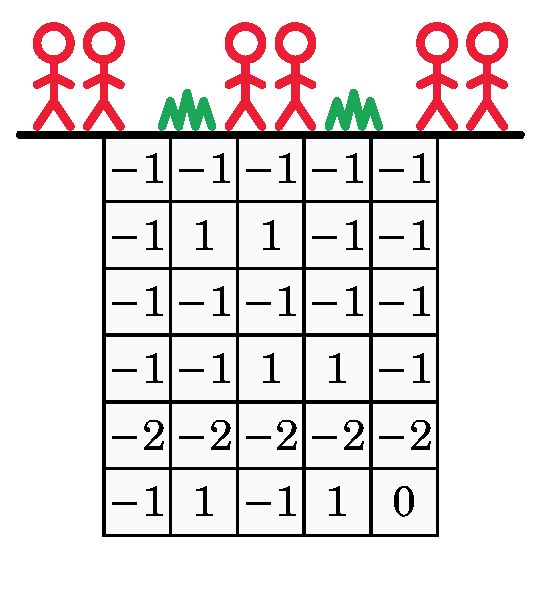
\includegraphics[scale=0.6]{figures/coding_descendingdrills_03.eps}
    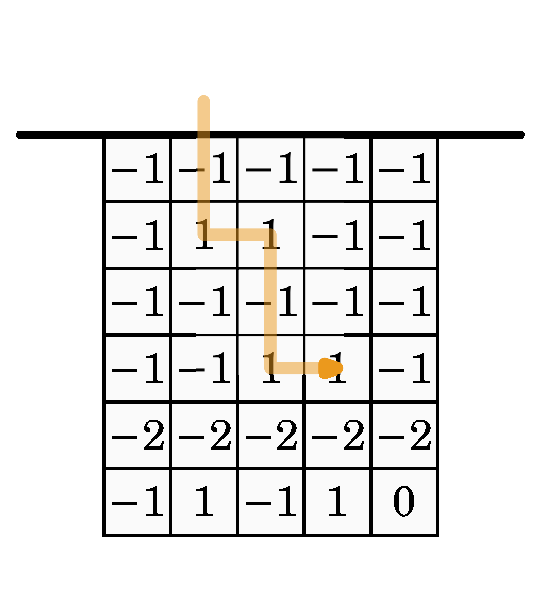
\includegraphics[scale=0.6]{figures/coding_descendingdrills_04.eps}
\end{center}

\subsection*{\sectionfont\upshape Constraints}

โปรแกรมของคุณจะถูกทดสอบกับ test cases สองชุด (เรียกว่าชุดเล็ก และชุดใหญ่)
\begin{itemize}
\item test cases ชุดเล็กจะมีเงื่อนไขว่า 
    ขนาดของตารางจะสอดคล้องกับเงื่อนไขที่ว่า \\ $1 \leq R, C \leq 200$
\item test cases ชุดใหญ่จะมีเงื่อนไขว่า 
    จำนวนช่องในตารางจะสอดคล้องกับเงื่อนไขที่ว่า \\ $1 \leq RC \leq 2 \cdot 10^6$
\item สำหรับทุก test cases จะมีเงื่อนไขว่า 
    จำนวนช่องที่ขยับได้ในแนวราบในแถว ๆ หนึ่งจะสอดคล้องกับเงื่อนไข $0 \leq K < C$ 
    และมูลค่าสมบัติแต่ละช่องจะมีค่าที่สอดคล้องกับเงื่อนไข 
    $-1000 \leq \text{\ttfamily v[i, j]} \leq 1000$
\end{itemize}
